% \section{Section Title}
\subsubsection{Μοντελοποίηση ενός νευρώνα}

Οι νευρώνες είναι εμπνευσμένοι από τους βιολογικούς νευρώνες του ανθρώπινου νευρικού συστήματος. Παρακάτω φαίνεται μια απεικόνιση ενός βιολογικού νευρώνα και η μαθηματική μοντελοποίησή του.\cite{cs231n} 

\begin{figure}[h]
\centering
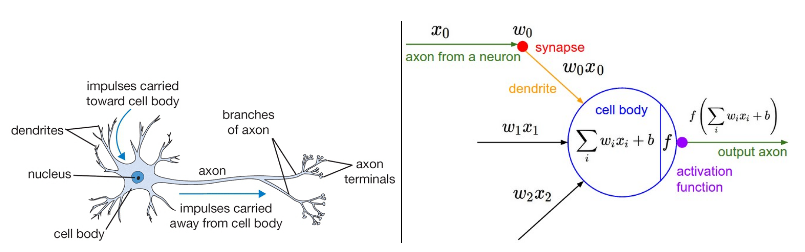
\includegraphics[scale=0.5]{images/Ch2/cs231n_neuron.png}
\caption{Μοντέλο Νευρώνα}
\label{fig:neuron model}
\end{figure}

Κάθε νευρώνας λαμβάνει σήματα από τους δενδρίτες και παράγει ένα σήμα εξόδου στον άξονα. Στη συνέχεια ο άξονας διακλαδίζεται μέσω συνάψεων σε δενδρίτες άλλων νευρώνων. Στο υπολογιστικό μοντέλο τα σήματα ($x_0$) στον άξονα, αλληλοεπιδρούν πολλαπλασιαστικά μέσω των συνάψεων με τους δενδρίτες ($w_0 x_0$) . Οι συνάψεις θεωρούμε πως είναι τα εκπαιδεύσιμα  στοιχεία (βάρη $w$)  τα οποία ελέγχουν την επιρροή του ενός νευρώνα σε κάποιον άλλο. Στο κυρίως μέρος του νευρώνα, αθροίζονται τα σήματα από τους δενδρίτες. Εάν αυτό το άθροισμα ξεπερνά ένα συγκεκριμένο κατώφλι, ο νευρώνας ενεργοποιείται και στέλνει σήμα στον άξονα εξόδου. Στο μαθηματικό μοντέλο ο ακριβής χρόνος που παράγονται τα σήματα δεν έχει σημασία, η συχνότητα ενεργοποίησης του νευρώνα μας ενδιαφέρει. Ο τρόπος με τον οποίο το αναπαριστούμε  αυτό είναι με μια συνάρτηση ενεργοποίησης. Η πιο συνηθισμένη συνάρτηση είναι η σιγμοειδής, η οποία έχει σαν είσοδο μια πραγματική τιμή (την ισχύ του σήματος μετά το άθροισμα) και το περιορίζει στο διάστημα μεταξύ 0 και 1. Με άλλα λόγια, κάθε νευρώνας εκτελεί το εσωτερικό γινόμενο της εισόδου με τα βάρη προσθέτοντας και μία σταθερά (\en{bias}) και εφαρμόζει μία μη γραμμική συνάρτηση, σε αυτή την περίπτωση η σιγμοειδής  $σ(x)=1/(1+e-x)$ .

\section{Νευρώνες}
Ο νευρώνας είναι μια απλή συνάρτηση. Παίρνει μία είσοδο $x$,  υπολογίζει μια συνάρτηση $f(x)$ και τις εξόδους της.  Επιλέγουμε τη λογιστική συνάρτηση:

\[ f(x)=\frac{1}{1+e^{-x}}\]

Η γραφική παράστασή της φαίνεται στο Σχήμα \ref{fig:logistic function}. Είναι η πιο συχνά χρησιμοποιούμενη συνάρτηση. Έχει την ιδιότητα ότι η έξοδός της είναι ουσιαστικά γραμμική ως προς την είσοδο, εάν το μέγεθος της εισόδου είναι μικρό. Αυτό σημαίνει ότι τα νευρωνικά δίκτυα με μικρά βάρη υπολογίζουν μια γραμμική συνάρτηση και η σταδιακή αύξηση των βαρών επιτρέπει τον έλεγχο της μη γραμμικότητας. Ο βαθμός της μη γραμμικότητας ελέγχει την "χωρητικότητα" του νευρωνικού δικτύου. Για παράδειγμα, ένα δίκτυο μόνο με γραμμικούς νευρώνες μπορεί να υπολογίσει μόνο γραμμικές συναρτήσεις

\begin{figure}[h]
\centering
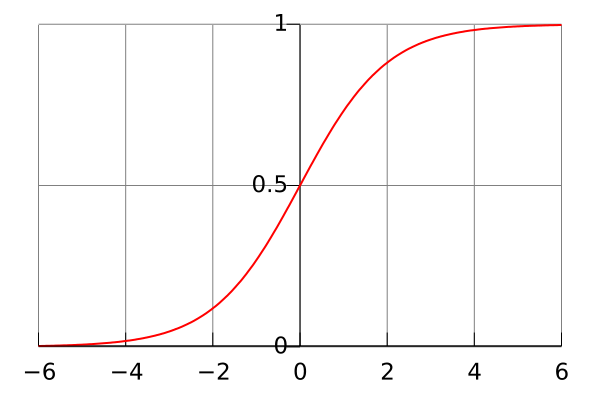
\includegraphics[scale=0.3]{images/Ch2/logistic-function.png}
\caption{Η λογιστική συνάρτηση $f(x)=\frac{1}{1+e^{-x}}$}
\label{fig:logistic function}
\end{figure}

\subsubsection{Νευρωνικό Δίκτυο Πρόσθιας Τροφοδότησης (\en{feed forward})}

\begin{figure}[h]
\centering
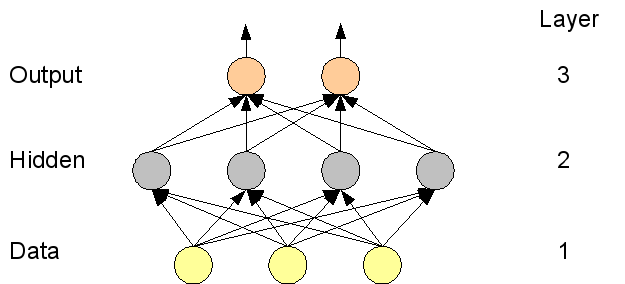
\includegraphics[scale=0.5]{images/Ch2/feed-forward.png}
\caption{\en{A feed-forward neural network with one hidden layer.}}
\label{fig:Feed Forward Neural Net}
\end{figure}

Τα \en{feed-forward} νευρωνικά δίκτυα συνδέουν μεταξύ τους επίπεδα νευρώνων. Κάθε νευρώνας  στο επίπεδο l συνδέεται με κάθε νευρώνα στο επίπεδο $l+1$, αλλά δεν υπάρχουν συνδέσεις εντός του επιπέδου. Αυτή η αρχιτεκτονική απεικονίζεται στο Σχήμα \ref{fig:Feed Forward Neural Net}.  Σε κάθε σύνδεση υπάρχει ένα βάρος με τιμές πραγματικούς αριθμούς. Ο νευρώνας k στο επίπεδο l δέχεται σαν είσοδο την τιμή:

$$
x_k^l=b_k^l+\sum_{i=1}^{N_{l-1}} w_{i k}^{l-1} y_i^{l-1}
$$

Όπου 
\begin{itemize}
    \item $b_k^l$   είναι το \en{bias} στον νευρώνα $k$ στο επίπεδο $l$,
    \item $N_{l-1}$ είναι ο αριθμός των νευρώνων στο επίπεδο $l-1$,
    \item $w_{ik}^{l-1}$  είναι το βάρος μεταξύ του νευρώνα $i$ στο επίπεδο $l-1$ και του νευρώνα $k$ στο επίπεδο $l$, και
    \item $y_{i}^{l-1}$    είναι η έξοδος του νευρώνα $i$ στο επίπεδο $l-1$
\end{itemize}
Στη συνέχεια ο νευρώνα υπολογίζει την έξοδο 

$$
y_k^l=f\left(x_k^l\right)
$$

Όπου $f$ είναι οποιαδήποτε διαφορίσιμη συνάρτηση του συνόλου των εισόδων του νευρώνα (εδώ η λογιστική συνάρτηση παραπάνω).  Οι νευρώνες στο επίπεδο \en{data}  έχουν σαν έξοδο απλά τα δεδομένα.
Τέλος, η συνάρτηση
$$
E\left(y_1^L, \ldots, y_{N_L}^L\right)
$$

της εξόδου του νευρωνικού δικτύου που θα θέλαμε να μεγιστοποιήσουμε (μπορούμε να το θεωρήσουμε σαν ένα επιπλέον επίπεδο στην έξοδο), όπου L είναι ο αριθμός των επιπέδων στο νευρωνικό δικτυο. Η Ε πρέπει να είναι διαφορίσιμη ώστε το $\frac{\partial{E}}{(\partial y_k^L}$    να είναι εύκολα υπολογίσιμο.
\en{Training the network consists of clamping the data neurons at the data and updating the parameters }
Η εκπαίδευση του νευρωνικού δικτύου περιλαμβάνει \en{clamping} τους νευρώνες δεδομένων με τα δεδομένα και ενημερώνοντας τις παραμέτρους (τα βάρη και των \en{biases}). Οι παράγωγοι υπολογίζονται με τον παρακάτω :

\begin{align*}
&\frac{\partial E}{\partial w_{i k}^{l-1}}=\frac{\partial E}{\partial x_k^l} y_i^{l-1}\\
&\frac{\partial E}{\partial b_k^l}=\frac{\partial E}{\partial x_k^l}\\
\end{align*}
Όπου 
\begin{align*}
&\frac{\partial E}{\partial x_k^l}=\frac{\partial E}{\partial y_k^l} \frac{\partial y_k^l}{\partial x_k^l}\\
&\frac{\partial E}{\partial y_k^l}= \begin{cases}\frac{\partial E}{\partial y_k^L} & \text { αν } l=L \\ \sum_{i=1}^{N_{l+1}} \frac{\partial E}{\partial x_i^{l+1}} w_{k i}^l & \text { αλλιώς }\end{cases}
\end{align*}

και το $\frac{\partial{E}}{\partial y_k^L}$  να είναι εύκολα υπολογίσιμο. Από αυτά, οι παράγωγοι ως προς τα βάρη και τα \en{bias} μπορούν να υπολογιστούν ξεκινώντας από το τελευταίο επίπεδο. Αυτό είναι γνωστό ως αλγόριθμος οπισθοδρομικής διάδοσης. 
Αν αυτό το δίκτυο χρησιμοποιηθεί για κατηγοριοποίηση, ο αριθμός των εξόδων ισούται με τον αριθμό των πιθανών κατηγοριών. Η έξοδος κάθε νευρώνα αντιστοιχεί στην εκτίμηση του δικτύου για κάποια κλάση.  

\subsubsection{Συνελικτικά Νευρωνικά Δίκτυα}
Στα συνηθισμένα νευρωνικά δίκτυα πρόσθιας διάδοσης, κάθε νευρώνας στο επίπεδο l συνδέεται με κάθε νευρώνα του επιπέδου $l-1$. Αυτό αρκεί αν δεν υπάρχουν τοπικές δομές στην ενεργοποίηση των νευρώνων του επιπέδου $l-1$. Όμως στην περίπτωση τον εικόνων υπάρχει κάποια δομή. Τα διπλανά \en{pixel} συσχετίζονται σε μεγαλύτερο βαθμό από αυτά που είναι μακριά. Για αυτό το λόγο κατευθύνουμε το νευρωνικό δίκτυο στην εξαγωγή τοπικών χαρακτηριστικών της εικόνας. Τα συνελικτικά δίκτυα το πετυχαίνουν αυτό συνδέοντας κάθε νευρώνα του κρυφού επιπέδου σε ένα μικρό σε ένα μικρό κομμάτι της εικόνας. Σε αυτή την περίπτωση επιλέγεται ένα κομμάτι 8\texttimes8. Ένα συνελικτικό δίκτυο με έναν νευρώνα θα εφαρμόσει αυτό το φίλτρο 8\texttimes8 σε όλες τις 33\texttimes33 πιθανές θέσεις μίας 32\texttimes32 εικόνας ( συμπληρώνοντας μηδενικά πλάτους 4 \en{pixel} σε κάθε άκρη). Οι έξοδοι των κρυμμένων επιπέδων αποτελούνται από εξόδους 33\texttimes33 αυτού του φίλτρου που εφαρμόζονται σε όλη την εικόνα. Σε αυτό το σημείο εμφανίζεται η συνέλιξη.

Το να έχουμε μόνο ένα νευρώνα είναι περιοριστικό, παρόλο που το φίλτρο εφαρμόζεται σε όλη την εικόνα και o νευρώνας έχει πάνω από χίλιες εξόδους. Θα θέλαμε να έχουμε πολλούς νευρώνες που μαθαίνουν διαφορετικά φίλτρα, καθένα εφαρμόζεται σε μια εικόνα. Αυτό το σενάριο απεικονίζεται στην εικόνα 3. Στην εικόνα υπάρχουν F κρυφοί νευρώνες συνολικά, και κάθε 32\texttimes32 πλάκα αναπαριστά τις εξόδους 32\texttimes32 που παράγονται από ένα κρυφό νευρώνα όπου κάνει συνέλιξη  το φίλτρο 8\texttimes8 με την εικόνα και εφαρμόζει την λογιστική συνάρτηση. Υπάρχουν 32\texttimes32 έξοδοι αντί για 33\texttimes33 επειδή στις \en{GPU} προτιμάμε αριθμούς όπως το 32 παρά το 33, και το νευρωνικό δίκτυο δεν θα χάσει αυτές τις λίγες επιπλέον εξόδους που λείπουν στις άκρες της εικόνας. Σε ένα τυπικό νευρωνικό δίκτυο για να πάρουμε 32\texttimes32 εξόδους από το κρυφό επίπεδο, θα πρέπει να έχουμε 32\texttimes32 νευρώνες σε αυτό ,  και αυτό επιτυγχάνεται εδώ με ένα μόνο νευρώνα. Έτσι μπορούμε να θεωρήσουμε τα συνελικτικά νευρωνικά δίκτυα σαν κανονικά νευρωνικά δίκτυα, αλλά με τον περιορισμό ότι ορισμένες ομάδες νευρώνων μοιράζονται τα βάρη (και επίσης οι αυτοί νευρώνες είναι μόνο τοπικά συνδεδεμένες με την εικόνα).

Οι έξοδοι ενός κρυφού νευρώνα όταν εφαρμόζεται συνέλιξη σε κοντινές περιοχές της εικόνας θα είναι παρόμοιες. Επομένως, η τιμές σε κοντινές περιοχές της ίδιας πλάκας 32\texttimes32 των εξόδων της κρυφής μονάδας (Σχήμα \ref{fig:cnn architecture}) στο κρυφό στρώμα είναι παρόμοιες. Έτσι, τα συνεπτυγμένα δίκτυα συχνά περιλαμβάνουν ένα στρώμα υποδειγματοληψίας ακριβώς πάνω από το συνεπτυγμένο στρώμα, για να υπολογίζεται τοπικά ο μέσος όρος των αποκρίσεων των κοντινών κρυφών μονάδων. Στο δίκτυό μου, οι μονάδες υπολογισμού του μέσου όρου υπολογίζουν τον μέσο όρο 4 \texttimes 4 μη επικαλυπτόμενων επιφανειών των εξόδων των κρυφών μονάδων. Το στρώμα υπολογισμού του μέσου όρου μειώνει το μέγεθος των πλακών των αποκρίσεων των κρυφών μονάδων από 32\texttimes32 σε 8 \texttimes 8. Μπορεί επίσης να υποστηριχθεί ότι η απώλεια κάποιας ακρίβειας όσον αφορά την ακριβή θέση των χαρακτηριστικών στην εικόνα είναι στην πραγματικότητα πλεονεκτική, επειδή επιτυγχάνεται μεγαλύτερος βαθμός αναλλοίωτης λειτουργίας. Στην όραση αποδεικνύεται συχνά ότι η ακριβής θέση ενός χαρακτηριστικού δεν είναι τόσο σημαντική όσο η κατά προσέγγιση θέση του σε σχέση με άλλα χαρακτηριστικά.

\begin{figure}[H]
\centering
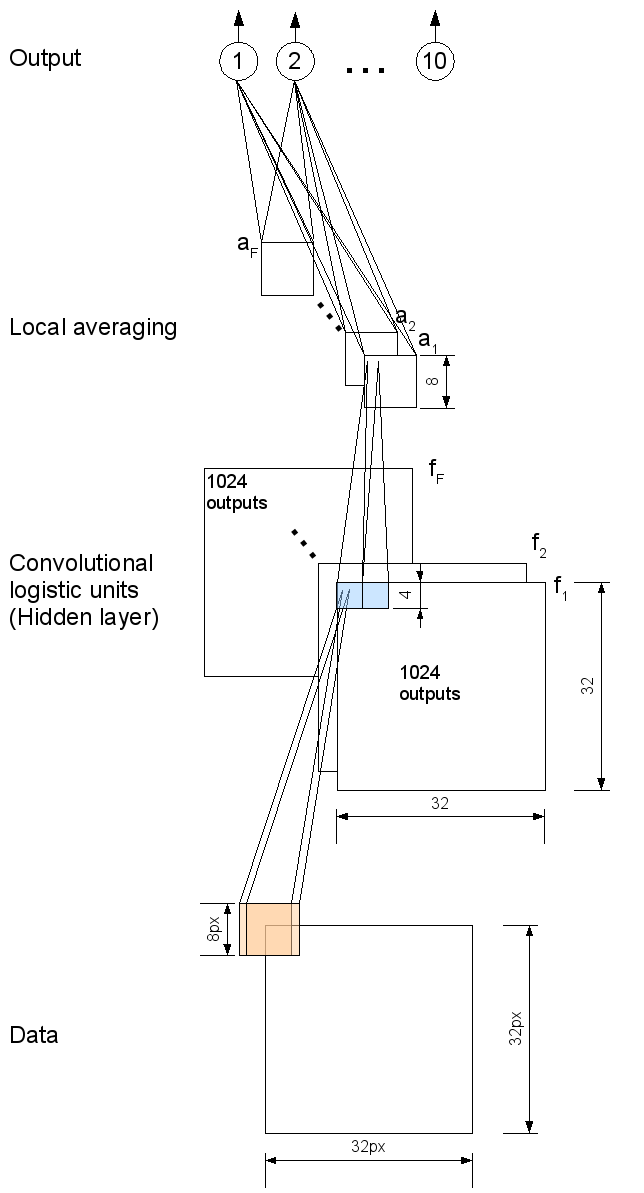
\includegraphics[width=0.5\textwidth]{images/Ch2/cnn-architecture.png}
\caption{\en{The architecture of the convolutional neural network.}}
\label{fig:cnn architecture}
\end{figure}

\section{Συνελικτικά νευρωνικά δίκτυα}
\en{ (CNNs / ConvNets})

πηγη:\en{ \url{https://cs231n.github.io/convolutional-networks/} }

Τα Συνελικτικά νευρωνικά δίκτυα μοιάζουν πολύ με τα συνηθισμένα Νευρωνικά Δίκτυα: αποτελούνται από νευρώνες που έχουν εκπαιδεύσιμα βάρη και σταθερές (\en{biases}).  Κάθε νευρώνας λαμβάνει κάποιες εισόδους, εκτελεί ένα εσωτερικό γινόμενο και προαιρετικά ακολουθεί μια μη γραμμικότητα. Ολόκληρο το δίκτυο εκφράζει μια ενιαία διαφορίσιμη συνάρτηση βαθμολογίας(\en{score}): από τα \en{pixel} μιας εικόνας στο ένα άκρο έως τις βαθμολογίες της κλάσης στο άλλο. Ακολουθεί μια συνάρτηση απωλειών (π.χ.\en{SVM/Softmax}) στο τελευταίο (πλήρως συνδεδεμένο) επίπεδο.

Οι αρχιτεκτονικές \en{ConvNet} κάνουν τη ρητή παραδοχή ότι οι είσοδοι είναι εικόνες, γεγονός που μας επιτρέπει να κωδικοποιήσουμε ορισμένες ιδιότητες στην αρχιτεκτονική. Αυτές στη συνέχεια καθιστούν πιο αποτελεσματική την υλοποίηση της συνάρτησης \en{forward} και μειώνουν κατά πολύ τον αριθμό των παραμέτρων στο δίκτυο.

\subsubsection{Επισκόπηση Αρχιτεκτονικής}

Τα απλά Νευρωνικά Δίκτυα λαμβάνουν μια είσοδο (ένα απλό διάνυσμα) και τη μετασχηματίζουν μέσω μιας σειράς κρυφών επιπέδων. Κάθε κρυφό επίπεδο αποτελείται από ένα σύνολο νευρώνων, όπου κάθε νευρώνας συνδέεται πλήρως με όλους τους νευρώνες του προηγούμενου επιπέδου και όπου οι νευρώνες ενός επιπέδου λειτουργούν εντελώς ανεξάρτητα και δεν μοιράζονται καμία σύνδεση. Το τελευταίο πλήρως συνδεδεμένο επίπεδο ονομάζεται "επίπεδο εξόδου" και αντιπροσωπεύει τις βαθμολογίες των κλάσεων.

Τα απλά Νευρωνικά Δίκτυα δεν προσαρμόζονται καλά (\en{don't scale}) σε πλήρεις εικόνες(\en{full images}). Στο \en{CIFAR-10}, οι εικόνες έχουν μέγεθος μόνο 32\texttimes32\texttimes3 (32 πλάτος, 32 ύψος, 3 χρωματικά κανάλια), οπότε ένας μόνο πλήρως συνδεδεμένος νευρώνας στο πρώτο κρυφό επίπεδο ενός κανονικού Νευρωνικού Δικτύου θα είχε 32*32*3 = 3072 βάρη. Αυτό το ποσό φαίνεται ακόμα διαχειρίσιμο, αλλά αυτή η πλήρως διασυνδεδεμένη δομή δεν κλιμακώνεται (\en{does not scale}) σε μεγαλύτερες εικόνες. Για παράδειγμα, μια εικόνα πιο μεγάλου μεγέθους, π.χ. 200\texttimes200\texttimes3, θα οδηγούσε σε νευρώνες που έχουν 200*200*3 = 120.000 βάρη. Επιπλέον, θα χρειαζόμασταν πολλούς  τέτοιους νευρώνες, οπότε οι παράμετροι θα αυξάνονταν κατά πολύ. Η πλήρης συνδεσιμότητα σε αυτή την περίπτωση κοστίζει σε όγκο και ο μεγάλος αριθμός παραμέτρων μπορεί  να οδηγήσει σε \en{overfitting}.

Τα Συνελικτικά Νευρωνικά Δίκτυα εκμεταλλεύονται το γεγονός ότι η είσοδος αποτελείται από εικόνες και χρησιμοποιούν την αρχιτεκτονική με τρόπο που έχει νόημα. Πιο συγκεκριμένα, σε αντίθεση με τα απλά Νευρωνικά Δίκτυα, τα επίπεδα του \en{ConvNet} έχουν νευρώνες οργανωμένους σε 3 διαστάσεις: πλάτος, ύψος, βάθος.( Με το βάθος αναφερόμαστε στην τρίτη διάσταση του όγκου ενεργοποίησης, όχι το βάθος ολόκληρου του Νευρωνικού Δικτύου, το οποίο αναφέρεται στον συνολικό αριθμό των επιπέδων στο δίκτυο.) Για παράδειγμα, οι εικόνες εισόδου στο \en{CIFAR-10} αποτελεί τον όγκο εισόδου των ενεργοποιήσεων, και ο όγκος έχει διαστάσεις 32\texttimes32\texttimes3 (πλάτος, ύψος, βάθος αντίστοιχα). 

Επιπλέον:\en{ \url{https://www.mathworks.com/discovery/convolutional-neural-network-matlab.html}}

\subsection{\en{Layers used to build ConvNets}}

\en{\url{https://cs231n.github.io/convolutional-networks/}}

Ένα απλό \en{ConvNet} είναι μια ακολουθία επιπέδων και κάθε επίπεδο ενός \en{ConvNet} μετατρέπει έναν όγκο ενεργοποιήσεων (\en{activations}) σε έναν άλλο μέσω μιας διαφορίσιμης συνάρτησης. Χρησιμοποιούμε τρεις βασικούς τύπους επιπέδων για την κατασκευή αρχιτεκτονικών \en{ConvNet : Convolutional Layer, Pooling Layer, και Fully-Connected Layer} (όπως και στα κανονικά νευρωνικά δίκτυα). 
Για παράδειγμα. Ένα απλό \en{ConvNet} για ταξινόμηση του \en{CIFAR-10}, θα μπορούσε να έχει την παρακάτω αρχιτεκτονική \en{[INPUT - CONV - RELU - POOL - FC]}, όπου:

\begin{itemize}
\item \en{INPUT} (Είσοδος) [32\texttimes32\texttimes3] περιέχει τις τιμές των \en{pixel} της εικόνας, στην περίπτωση μας μία εικόνα πλάτους 32, ύψους 32 και τρία κανάλια χρωμάτων \en{R,G,B}.
\item \en{CONV layer} (Συνελικτικό επίπεδο) υπολογίζει την έξοδο των νευρώνων που συνδέονται τοπικά σε περιοχές της εικόνας εισόδου, καθένας υπολογίζει το εσωτερικό γινόμενο από τα βάρη και μια μικρή περιοχή που συνδέεται στην είσοδο του όγκου. Αυτό θα έχει σαν αποτέλεσμα έναν όγκο [32\texttimes32\texttimes12] εάν αποφασίσουμε να χρησιμοπιοήσουμε 12 φίλτρα.
\item \en{RELU layer} (επίπεδο συνάρτησης \en{ReLu}) σε κάθε στοιχείο εφαρμόζεται μια συνάρτηση ενεργοποίησης ,όπως η \en{max(0,x)} με κατώφλι στο 0. Αυτό το επίπεδο αφήνει το μέγεθος του όγκου το ίδιο ([32\texttimes32\texttimes12]).
\item \en{POOL layer} αυτό το επίπεδο εκτελεί μια πράξη υποδειγματοληψίας κατά μήκος των χωρικών διαστάσεων (πλάτος, ύψος), με αποτέλεσμα έναν όγκο [16\texttimes16\texttimes12].
\item \en{FC (i.e. fully-connected) layer} (Πλήρως διασυνδεμένο επίπεδο) θα υπολογίσει τις βαθμολογίες των κλάσσεων, με αποτέλεσμα έναν όγκο μεγέθους [1\texttimes1\texttimes10], όπου κάθε ένας από τους 10 αριθμούς αντιστοιχεί στη βαθμολογία μιας κλάσης αναμεσα στις 10 κατηγορίες του \en{CIFAR-10}. Όπως και στα συνηθισμένα Νευρωνικά Δίκτυα και όπως υποδηλώνει το όνομα, κάθε νευρώνας σε αυτό το επίπεδο συνδέεται με όλους τους αριθμούς του προηγούμενου όγκου.
\end{itemize}

Με αυτό τον τρόπο, τα \en{ConvNets} μετατρέπουν μια εικόνα, \en{ layer by layer from the original \en{pixel} values to the final class scores. Note that some layers contain parameters and other don’t. In particular, the CONV/FC layers perform transformations that are a function of not only the activations in the input volume, but also of the parameters (the weights and biases of the neurons). On the other hand, the RELU/POOL layers will implement a fixed function. The parameters in the CONV/FC layers will be trained with gradient descent so that the class scores that the ConvNet computes are consistent with the labels in the training set for each image.}\\

\noindent
\en{In summary:
    \begin{itemize}
    \item A ConvNet architecture is in the simplest case a list of Layers that transform the image volume into an output volume (e.g. holding the class scores)
    \item There are a few distinct types of Layers (e.g. CONV/FC/RELU/POOL are by far the most popular)
    \item Each Layer accepts an input 3D volume and transforms it to an output 3D volume through a differentiable function
    \item Each Layer may or may not have parameters (e.g. CONV/ FC do, RELU/ POOL don’t)
    \item Each Layer may or may not have additional hyperparameters (e.g. CONV/ FC/ POOL do, RELU doesn’t)
    \end{itemize}
}